\section{Proposed questions}

\section*{Part A: Clustering}

\subsection{Question 1}
\textbf{Do clustering-guided summarization alters the behavior and efficacy of the IR system?}

To answer this question we ran the \textbf{clustering based} algorithm using
the same set of documents used in the \textit{first part of the project}. The
result shows a pretty big difference between the two approaches.

% do a minipage fo r2 figurs
\begin{figure}[H]
  \centering
  \begin{minipage}{.5\textwidth}
    \centering
    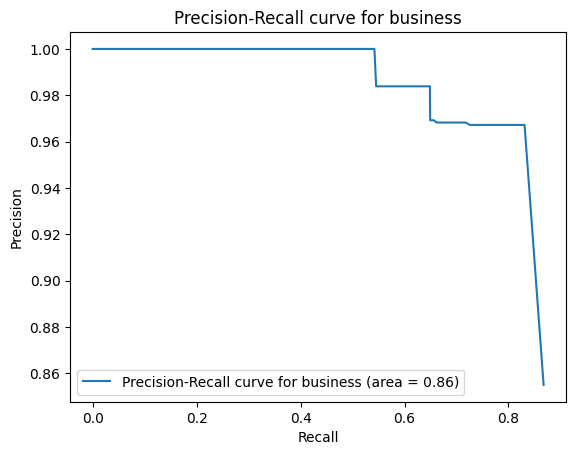
\includegraphics[width=1\linewidth]{images/pr_question_1_part1.png}
    \captionof{figure}{First Part Approach}
    \label{fig:firstpart}
  \end{minipage}%
  \begin{minipage}{.5\textwidth}
    \centering
    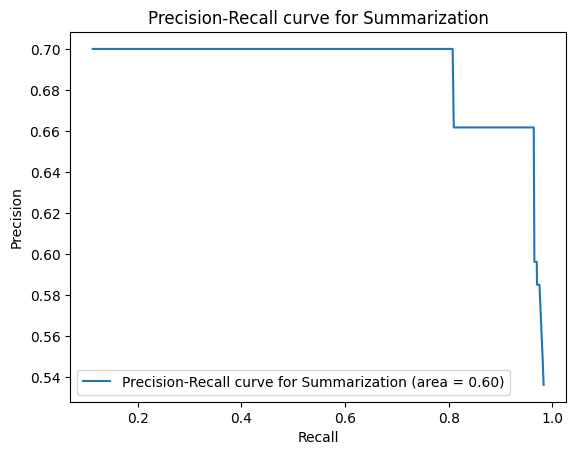
\includegraphics[width=1\linewidth]{images/pr_question_1.png}
    \captionof{figure}{Clustered Approach}
    \label{fig:clustered}
  \end{minipage}
\end{figure}

This result doesn't guarantee that the \textbf{clustering based} approach is
worse than the approach using TFIDF and BM25, because this is based on our
personal implementation of the algorithm. However, it is clear that the
clustering approach is not as effective as the first approach in this case. A
possible way to improve the algorithm could be to consider other sentences
choices rather than focusing on the distance from the centroid of each cluster.

\subsection{Question 2}
\textbf{How sentence representations, clustering choices, and rank criteria impact summarization?}

We benchmarked the performance of the clustering algorithm using a set of
metrics:
\begin{table}[H]
  \centering
  \begin{tabular}{|c|c|c|}
    \hline
    \textbf{Max Clusters} & \textbf{Number of Sentences} & \textbf{Our Metrics} \\
    \hline
    2                     & 3                            &                      \\
    3                     & 5                            &                      \\
    4                     & 7                            & cosine               \\
    6                     & 9                            & euclidean            \\
    8                     & 11                           &                      \\
    10                    & 13                           &                      \\
    \hline
  \end{tabular}
\end{table}

We didn't include any \textbf{different representations} because we only used
the \textbf{TFIDF} representation. The result are indicating a very low
performance of the algorithm using a specific set of metrics.

\begin{table}[H]
  \centering
  \caption{Results of the clustering algorithm using different metrics}
  \label{tab:my-table}
  \begin{tabular}{|c|c|c|c|c|c|c|c|}
    \hline
    \textbf{\#cluters} & \textbf{\#sentences} & \textbf{metric} & \textbf{avg\_prec} & \textbf{avg\_rec} & \textbf{f1} & \textbf{m\_a\_p} \\ \hline
    2                      & 3                              & cosine          & 0.453504                    & 0.449012                 & 0.451247    & 0.646069         \\ \hline
    2                      & 3                              & euclidean       & 0.453504                    & 0.449012                 & 0.451247    & 0.646069         \\ \hline
    2                      & 5                              & cosine          & 0.457060                    & 0.633170                 & 0.530891    & 0.561392         \\ \hline
    2                      & 5                              & euclidean       & 0.457060                    & 0.633170                 & 0.530891    & 0.561392         \\ \hline
    2                      & 7                              & cosine          & 0.469898                    & 0.768889                 & 0.583312    & 0.492352         \\ \hline
    ...                    & ...                            & ...             & ...                         & ...                      & ...         & ...              \\ \hline
    10                     & 9                              & euclidean       & 0.484872                    & 0.934921                 & 0.638568    & 0.418472         \\ \hline
    10                     & 11                             & cosine          & 0.486431                    & 0.941682        
             & 0.641495    & 0.344811         \\ \hline
    10                     & 11                             & euclidean       & 0.486431                    & 0.941682                 & 0.641495    & 0.344811         \\ \hline
    10                     & 13                             & cosine          & 0.486635                    & 0.943571                 & 0.642110    & 0.336604         \\ \hline
    10                     & 13                             & euclidean       & 0.486635                    & 0.943571                 & 0.642110    & 0.336604         \\ \hline
  \end{tabular}
\end{table}

More insight on this can be found in the \textit{notebook} file.


\subsection{Question 3}
\textbf{ Are anchor sentences (capturing multiple topics) included? And less relevant outlier sen- tences excluded? Justify}

Since our algorithm is based on the \textbf{distance from the centroid} of each cluster to select the sentences, 
we are not able to handle the \textbf{anchor sentences} and the \textbf{outlier sentences}. We are not able to give a clear answer to this question, but 
a possible way to handle this could be to consider the \textbf{distance from the centroid} and the \textbf{distance from the other sentences} inside other clusters. 
Sentences that are \textbf{more far} from the centroid of the cluster could be very \textbf{relevant} and could be considered as \textbf{anchor sentences}, since that 
sentence could be holding information between more topics. 

\subsection{Question 4}
\textbf{Given a set of documents, plot the distribution of the number of keywords per document. Are keywords generally dissimilar? If not, how would you tackle this challenge?}
For this question we decided to use documents from \[500,700\] as range. The result shows that the distribution of the number of keywords per document is not uniform.

\begin{figure}[H]
  \begin{minipage}{.5\textwidth}
    \centering
    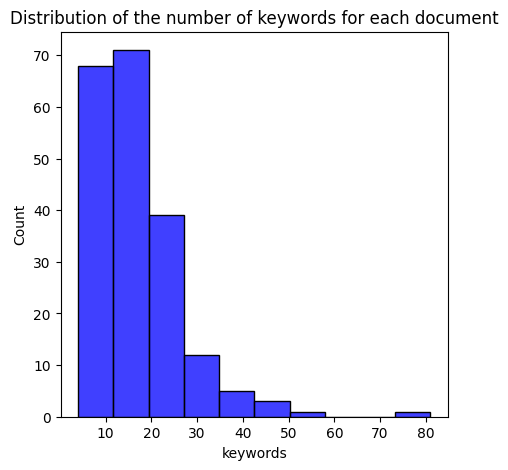
\includegraphics[width=1\linewidth]{images/keyword_distribution.png}
    \captionof{figure}{Distribution of the number of keywords per document}
    \label{fig:question4_1}
  \end{minipage}
  \begin{minipage}{.5\textwidth}
    \centering
    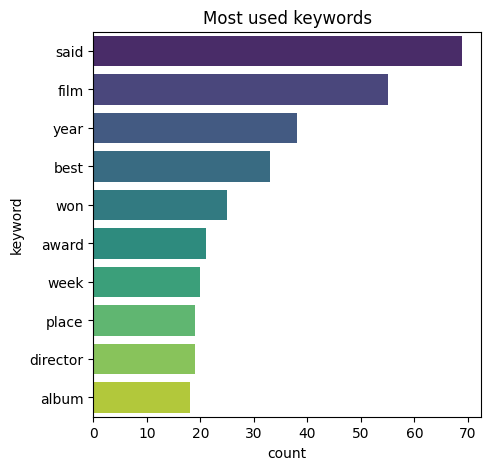
\includegraphics[width=1\linewidth]{images/keyword_distribution_ranks.png}
    \captionof{figure}{Distribution of the number of keywords per document}
    \label{fig:question4_2}
  \end{minipage}
\end{figure}

\section*{Part B: Supervised IR}
\subsection{Question 1}
\textbf{ Does the incorporation of relevance feedback from ideal extracts significantly impact the performance of the IR system? Hypothesize why is that so.}

\subsection{Question 2}
\textbf{ Are the learned models able to generalize from one category to another? Justify.}
\subsection{Question 3}

\textbf{Which features appear to be more relevant to the target summarization task? Do sentence- location features aid summarization?}

\subsection{Question 4}
\textbf{In alternative to the given reference extracts, consider the presence of manual abstractive summaries, can supervised IR be used to explore such feedback? Justify}

